\documentclass[journal,12pt,twocolumn]{IEEEtran}
%
\usepackage{setspace}
\usepackage{gensymb}
\usepackage{xcolor}
\usepackage{caption}
%\usepackage{subcaption}
%\doublespacing
\singlespacing

%\usepackage{graphicx}
%\usepackage{amssymb}
%\usepackage{relsize}
\usepackage[cmex10]{amsmath}
\usepackage{mathtools}
%\usepackage{amsthm}
%\interdisplaylinepenalty=2500
%\savesymbol{iint}
%\usepackage{txfonts}
%\restoresymbol{TXF}{iint}
%\usepackage{wasysym}
\usepackage{hyperref}
\usepackage{amsthm}
\usepackage{mathrsfs}
\usepackage{txfonts}
\usepackage{stfloats}
\usepackage{cite}
\usepackage{cases}
\usepackage{subfig}
%\usepackage{xtab}
\usepackage{longtable}
\usepackage{multirow}
%\usepackage{algorithm}
%\usepackage{algpseudocode}
%\usepackage{enumerate}
\usepackage{enumitem}
\usepackage{mathtools}
%\usepackage{iithtlc}
%\usepackage[framemethod=tikz]{mdframed}
\usepackage{listings}


%\usepackage{stmaryrd}


%\usepackage{wasysym}
%\newcounter{MYtempeqncnt}
\DeclareMathOperator*{\Res}{Res}
%\renewcommand{\baselinestretch}{2}
\renewcommand\thesection{\arabic{section}}
\renewcommand\thesubsection{\thesection.\arabic{subsection}}
\renewcommand\thesubsubsection{\thesubsection.\arabic{subsubsection}}

\renewcommand\thesectiondis{\arabic{section}}
\renewcommand\thesubsectiondis{\thesectiondis.\arabic{subsection}}
\renewcommand\thesubsubsectiondis{\thesubsectiondis.\arabic{subsubsection}}

%\renewcommand{\labelenumi}{\textbf{\theenumi}}
%\renewcommand{\theenumi}{P.\arabic{enumi}}

% correct bad hyphenation here
\hyphenation{op-tical net-works semi-conduc-tor}

\lstset{
language=Python,
frame=single, 
breaklines=true,
columns=fullflexible
}



\begin{document}
%

\theoremstyle{definition}
\newtheorem{theorem}{Theorem}[section]
\newtheorem{problem}{Problem}
\newtheorem{proposition}{Proposition}[section]
\newtheorem{lemma}{Lemma}[section]
\newtheorem{corollary}[theorem]{Corollary}
\newtheorem{example}{Example}[section]
\newtheorem{definition}{Definition}[section]
%\newtheorem{algorithm}{Algorithm}[section]
%\newtheorem{cor}{Corollary}
\newcommand{\BEQA}{\begin{eqnarray}}
\newcommand{\EEQA}{\end{eqnarray}}
\newcommand{\define}{\stackrel{\triangle}{=}}

\bibliographystyle{IEEEtran}
%\bibliographystyle{ieeetr}

\providecommand{\nCr}[2]{\,^{#1}C_{#2}} % nCr
\providecommand{\nPr}[2]{\,^{#1}P_{#2}} % nPr
\providecommand{\mbf}{\mathbf}
\providecommand{\pr}[1]{\ensuremath{\Pr\left(#1\right)}}
\providecommand{\qfunc}[1]{\ensuremath{Q\left(#1\right)}}
\providecommand{\sbrak}[1]{\ensuremath{{}\left[#1\right]}}
\providecommand{\lsbrak}[1]{\ensuremath{{}\left[#1\right.}}
\providecommand{\rsbrak}[1]{\ensuremath{{}\left.#1\right]}}
\providecommand{\brak}[1]{\ensuremath{\left(#1\right)}}
\providecommand{\lbrak}[1]{\ensuremath{\left(#1\right.}}
\providecommand{\rbrak}[1]{\ensuremath{\left.#1\right)}}
\providecommand{\cbrak}[1]{\ensuremath{\left\{#1\right\}}}
\providecommand{\lcbrak}[1]{\ensuremath{\left\{#1\right.}}
\providecommand{\rcbrak}[1]{\ensuremath{\left.#1\right\}}}
\theoremstyle{remark}
\newtheorem{rem}{Remark}
\newcommand{\sgn}{\mathop{\mathrm{sgn}}}
\providecommand{\abs}[1]{\left\vert#1\right\vert}
\providecommand{\res}[1]{\Res\displaylimits_{#1}} 
\providecommand{\norm}[1]{\lVert#1\rVert}
\providecommand{\mtx}[1]{\mathbf{#1}}
\providecommand{\mean}[1]{E\left[ #1 \right]}
\providecommand{\fourier}{\overset{\mathcal{F}}{ \rightleftharpoons}}
\providecommand{\ztrans}{\overset{\mathcal{Z}}{ \rightleftharpoons}}

%\providecommand{\hilbert}{\overset{\mathcal{H}}{ \rightleftharpoons}}
\providecommand{\system}{\overset{\mathcal{H}}{ \longleftrightarrow}}
	%\newcommand{\solution}[2]{\textbf{Solution:}{#1}}
\newcommand{\solution}{\noindent \textbf{Solution: }}
\providecommand{\dec}[2]{\ensuremath{\overset{#1}{\underset{#2}{\gtrless}}}}
\numberwithin{equation}{section}
%\numberwithin{equation}{subsection}
%\numberwithin{problem}{subsection}
%\numberwithin{definition}{subsection}
\makeatletter
\@addtoreset{figure}{problem}
\makeatother

\let\StandardTheFigure\thefigure
%\renewcommand{\thefigure}{\theproblem.\arabic{figure}}
\renewcommand{\thefigure}{\theproblem}


%\numberwithin{figure}{subsection}

\def\putbox#1#2#3{\makebox[0in][l]{\makebox[#1][l]{}\raisebox{\baselineskip}[0in][0in]{\raisebox{#2}[0in][0in]{#3}}}}
     \def\rightbox#1{\makebox[0in][r]{#1}}
     \def\centbox#1{\makebox[0in]{#1}}
     \def\topbox#1{\raisebox{-\baselineskip}[0in][0in]{#1}}
     \def\midbox#1{\raisebox{-0.5\baselineskip}[0in][0in]{#1}}

\vspace{3cm}

\title{ 
%\logo{
Digital Signal Processing
%}
%	\logo{Octave for Math Computing }
}
%\title{
%	\logo{Matrix Analysis through Octave}{\begin{center}\includegraphics[scale=.24]{tlc}\end{center}}{}{HAMDSP}
%}


% paper title
% can use linebreaks \\ within to get better formatting as desired
%\title{Matrix Analysis through Octave}
%
%
% author names and IEEE memberships
% note positions of commas and nonbreaking spaces ( ~ ) LaTeX will not break
% a structure at a ~ so this keeps an author's name from being broken across
% two lines.
% use \thanks{} to gain access to the first footnote area
% a separate \thanks must be used for each paragraph as LaTeX2e's \thanks
% was not built to handle multiple paragraphs
%

\author{ G V V Sharma$^{*}$ %<-this  stops a space
\thanks{*The author is with the Department
of Electrical Engineering, Indian Institute of Technology, Hyderabad
502285 India e-mail:  gadepall@iith.ac.in.  All content in the manuscript is 
released under GNU GPL.  Free to use for anything. }% <-this % stops a space
%\thanks{J. Doe and J. Doe are with Anonymous University.}% <-this % stops a space
%\thanks{Manuscript received April 19, 2005; revised January 11, 2007.}}
}
% note the % following the last \IEEEmembership and also \thanks - 
% these prevent an unwanted space from occurring between the last author name
% and the end of the author line. i.e., if you had this:
% 
% \author{....lastname \thanks{...} \thanks{...} }
%                     ^------------^------------^----Do not want these spaces!
%
% a space would be appended to the last name and could cause every name on that
% line to be shifted left slightly. This is one of those "LaTeX things". For
% instance, "\textbf{A} \textbf{B}" will typeset as "A B" not "AB". To get
% "AB" then you have to do: "\textbf{A}\textbf{B}"
% \thanks is no different in this regard, so shield the last } of each \thanks
% that ends a line with a % and do not let a space in before the next \thanks.
% Spaces after \IEEEmembership other than the last one are OK (and needed) as
% you are supposed to have spaces between the names. For what it is worth,
% this is a minor point as most people would not even notice if the said evil
% space somehow managed to creep in.



% The paper headers
%\markboth{Journal of \LaTeX\ Class Files,~Vol.~6, No.~1, January~2007}%
%{Shell \MakeLowercase{\textit{et al.}}: Bare Demo of IEEEtran.cls for Journals}
% The only time the second header will appear is for the odd numbered pages
% after the title page when using the twoside option.
% 
% *** Note that you probably will NOT want to include the author's ***
% *** name in the headers of peer review papers.                   ***
% You can use \ifCLASSOPTIONpeerreview for conditional compilation here if
% you desire.




% If you want to put a publisher's ID mark on the page you can do it like
% this:
%\IEEEpubid{0000--0000/00\$00.00~\copyright~2007 IEEE}
% Remember, if you use this you must call \IEEEpubidadjcol in the second
% column for its text to clear the IEEEpubid mark.



% make the title area
\maketitle

%\newpage

\tableofcontents

%\renewcommand{\thefigure}{\thesection.\theenumi}
%\renewcommand{\thetable}{\thesection.\theenumi}

\renewcommand{\thefigure}{\theenumi}
\renewcommand{\thetable}{\theenumi}

%\renewcommand{\theequation}{\thesection}


\bigskip

\begin{abstract}
This manual provides a simple introduction to digital signal processing.
\end{abstract}
\section{Software Installation}
Run the following commands
\begin{lstlisting}
sudo apt-get update
sudo apt-get install libffi-dev libsndfile1 python3-scipy  python3-numpy python3-matplotlib 
sudo pip install cffi pysoundfile 
\end{lstlisting}
\section{Digital Filter}
\begin{enumerate}[label=\thesection.\arabic*
,ref=\thesection.\theenumi]
\item
\label{prob:input}
Download the sound file from  
\begin{lstlisting}
wget https://raw.githubusercontent.com/gadepall/ 
EE1310/master/filter/codes/Sound_Noise.wav
\end{lstlisting}
%\href{http://tlc.iith.ac.in/img/sound/Sound_Noise.wav}{\url{http://tlc.iith.ac.in/img/sound/Sound_Noise.wav}}  
%in the link given below.
%\linebreak
\item
\label{prob:spectrogram}
You will find a spectrogram at \href{https://academo.org/demos/spectrum-analyzer}{\url{https://academo.org/demos/spectrum-analyzer}}. 
%\end{problem}
%%
%
%%\onecolumn
%%\input{./figs/fir}
%\begin{problem}
Upload the sound file that you downloaded in Problem \ref{prob:input} in the spectrogram  and play.  Observe the spectrogram. What do you find?
\\
%
\solution There are a lot of yellow lines between 440 Hz to 5.1 KHz.  These represent the synthesizer key tones. Also, the key strokes
are audible along with background noise.
% By observing spectrogram, it clearly shows that tonal frequency is under 4kHz. And above 4kHz only noise is present.
\item
\label{prob:output}
Write the python code for removal of out of band noise and execute the code.
\\
\solution
\begin{lstlisting}
wget https://github.com/Bhanu-das/EE3900-2022/blob/main/filter/codes/Cancel_noise.py
\end{lstlisting}
%\begin{figure}[h]
%\centering
%\includegraphics[width=\columnwidth]{enc_block_diag.png}
%\caption{}
%\label{fig:convolution encoder}
%\end{figure}
%\input{block_enc}
\item
The output of the python script in Problem \ref{prob:output} is the audio file Sound\_With\_ReducedNoise.wav. Play the file in the spectrogram in Problem \ref{prob:spectrogram}. What do you observe?
\\
\solution The key strokes as well as background noise is subdued in the audio.  Also,  the signal is blank for frequencies above 5.1 kHz.

\end{enumerate}
\section{Difference Equation}
\begin{enumerate}[label=\thesection.\arabic*,ref=\thesection.\theenumi]
\item Let
	\label{def:xn}
\begin{equation}
x(n) = \cbrak{\underset{\uparrow}{1},2,3,4,2,1}
\end{equation}
Sketch $x(n)$.
\newline
\solution
python code
\begin{lstlisting}
weget https://github.com/Bhanu-das/EE3900/blob/main/Assign1/codes/Q3/X_Y.py
\end{lstlisting}
sketch
\begin{lstlisting}
weget https://github.com/Bhanu-das/EE3900/blob/main/Assign1/fig/Q3.png
\end{lstlisting}
\item Let
\begin{multline}
\label{eq:iir_filter}
y(n) + \frac{1}{2}y(n-1) = x(n) + x(n-2), 
\\
 y(n) = 0, n < 0
\end{multline}
Sketch $y(n)$.  
\\
\solution The following code yields Fig. {fig:xnyn}.
\begin{lstlisting}
wget https://github.com/gadepall/EE1310/raw/master/filter/codes/xnyn.py
\end{lstlisting}
\begin{lstlisting}
wget https://github.com/Bhanu-das/EE3900-2022/blob/main/filter/figs/xnyn.pdf
\end{lstlisting}

\item Repeat the above exercise using a C code.
\newline
\solution c code
\begin{lstlisting}
weget https://github.com/Bhanu-das/EE3900/blob/main/Assign1/codes/Q3/x_y.c
\end{lstlisting}
\end{enumerate}
\section{$Z$-transform}
\begin{enumerate}[label=\thesection.\arabic*]
\item The $Z$-transform of $x(n)$ is defined as
%
\begin{equation}
\label{eq:z_trans}
X(z)={\mathcal {Z}}\{x(n)\}=\sum _{n=-\infty }^{\infty }x(n)z^{-n}
\end{equation}
%
Show that
\begin{equation}
\label{eq:shift1}
{\mathcal {Z}}\{x(n-1)\} = z^{-1}X(z)
\end{equation}
and find
\begin{equation}
	{\mathcal {Z}}\{x(n-k)\} 
\end{equation}
\solution From \eqref{eq:z_trans},
\begin{align}
{\mathcal {Z}}\{x(n-k)\} &=\sum _{n=-\infty }^{\infty }x(n-1)z^{-n}
\\
&=\sum _{n=-\infty }^{\infty }x(n)z^{-n-1} = z^{-1}\sum _{n=-\infty }^{\infty }x(n)z^{-n}
\end{align}
resulting in \eqref{eq:shift1}. Similarly, it can be shown that
%
\begin{equation}
\label{eq:z_trans_shift}
	{\mathcal {Z}}\{x(n-k)\} = z^{-k}X(z)
\end{equation}
\item Obtain $X(z)$ for $x(n)$ defined in problem 
	\ref{def:xn}.
\solution
\begin{equation}
    X(z) = \sum_{n=-\infty}^{\infty}x(n)z^{-n}
\end{equation}
But
\begin{equation}
    x(n) = \cbrak{1,2,3,4,2,1}
\end{equation}
so,
\begin{equation}
    X(z) = 1 + 2z^{-1} + 3z^{-2} + 4z^{-3} + 2z^{-4} + z^{-5}
\end{equation}
\item Find
%
\begin{equation}
H(z) = \frac{Y(z)}{X(z)}
\end{equation}
%
from  \eqref{eq:iir_filter} assuming that the $Z$-transform is a linear operation.
\\
\solution  Applying \eqref{eq:z_trans_shift} in \eqref{eq:iir_filter},
\begin{align}
Y(z) + \frac{1}{2}z^{-1}Y(z) &= X(z)+z^{-2}X(z)
\\
\implies \frac{Y(z)}{X(z)} &= \frac{1 + z^{-2}}{1 + \frac{1}{2}z^{-1}}
\label{eq:freq_resp}
\end{align}
%
\item Find the Z transform of 
\begin{equation}
\delta(n)
=
\begin{cases}
1 & n = 0
\\
0 & \text{otherwise}
\end{cases}
\end{equation}
and show that the $Z$-transform of
\begin{equation}
\label{eq:unit_step}
u(n)
=
\begin{cases}
1 & n \ge 0
\\
0 & \text{otherwise}
\end{cases}
\end{equation}
is
\begin{equation}
U(z) = \frac{1}{1-z^{-1}}, \quad \abs{z} > 1
\end{equation}
\solution It is easy to show that
\begin{equation}
\delta(n) \ztrans 1
\end{equation}
and from \eqref{eq:unit_step},
\begin{align}
U(z) &= \sum _{n= 0}^{\infty}z^{-n}
\\
&=\frac{1}{1-z^{-1}}, \quad \abs{z} > 1
\end{align}
using the fomula for the sum of an infinite geometric progression.
%
\item Show that 
\begin{equation}
\label{eq:anun}
a^nu(n) \ztrans \frac{1}{1-az^{-1}} \quad \abs{z} > \abs{a}
\end{equation}
\solution
\textbf{Solution: }
let
\begin{equation}
    f(n) = a^n u(n)
\end{equation}
\begin{equation}
f(n) = 
\left\{
    \begin{array}{lr}
        a^n, & \text{if } n>0\\
        0  , & \text{otherwise}
    \end{array}
\right\}
\end{equation}
Now the Z- Transform of f(n) is
\begin{equation}
    F(z) = {\mathcal {Z}}\{f(n)\} = \sum_{n=-\infty}^{\infty} f(n)z^{-n}
\end{equation}
\begin{equation}
    F(z) = \sum_{n=0}^{\infty} a^{n}z^{-n}
\end{equation}
This forms a infinite Geometric Progression.
\begin{equation}
    F(z) = \frac{1}{1-az^{-1}} \text{ for } z<a.
\end{equation}

%
\item 
Let
\begin{equation}
H\brak{e^{\j \omega}} = H\brak{z = e^{j \omega}}.
\end{equation}
Plot $\abs{H\brak{e^{j \omega}}}$.  Is it periodic? If so, find the period. $H(e^{\j \omega})$ is
known as the {\em Discret Time Fourier Transform} (DTFT) of $h(n)$.
\\
\solution The following code plots 
\begin{lstlisting}
wget https://raw.githubusercontent.com/gadepall/EE1310/master/filter/codes/dtft.py
\end{lstlisting}
\begin{lstlisting}
wget https://github.com/Bhanu-das/EE3900-2022/blob/main/filter/figs/dtft.pdf
\end{lstlisting}
\item Express $h(n)$ in terms of $H\brak{e^{\j \omega}}$.
\solution We have,
\begin{align}
	H(e^{\j\omega}) &= \sum_{k = -\infty}^{\infty}h(k)e^{-\j\omega k}
\end{align}
However,
\begin{align}
	\int_{-\pi}^{\pi}e^{\j\omega(n - k)}d\omega =
	\begin{cases}
		2\pi & n = k \\
		0 & \textrm{otherwise}
	\end{cases}
\end{align}
and so,
\begin{align}
	&\frac{1}{2\pi}\int_{-\pi}^{\pi}H(e^{\j\omega})e^{j\omega n}d\omega \\
	&= \frac{1}{2\pi}\sum_{k = -\infty}^{\infty}\int_{-\pi}^{\pi}h(k)e^{\j\omega(n - k)}d\omega \\
	&= \frac{1}{2\pi}2\pi h(n) = h(n)
\end{align}
which is known as the Inverse Discrete Fourier Transform. Thus,
\begin{align}
	h(n) &= \frac{1}{2\pi}\int_{-\pi}^{\pi}H(e^{\j\omega})e^{\j\omega n}d\omega \\
		 &= \frac{1}{2\pi}\int_{-\pi}^{\pi}\frac{1 + e^{-2\j\omega}}{1 + \frac{1}{2}e^{-\j\omega}}e^{\j\omega n}d\omega
	\label{eq:idtft}
\end{align}

\end{enumerate}

\section{Impulse Response}
\begin{enumerate}[label=\thesection.\arabic*]
	\item Using long division, 
find
		\begin{align}
			h(n), \quad n < 5
		\end{align}
		for H(z) in 
		\eqref{eq:freq_resp}.
\solution from \eqref{eq:freq_resp}
\begin{equation}
    H(z) = \frac{1 + z^{-2}}{1 + \frac{1}{2}z^{-1}}
\end{equation}
\begin{center}
    $1 + \frac{1}{2}z^{-1}\overline{)1 + z^{-2}(} 2z^{-1}$\\
    ${2z^{-1} + z^{-2}}$\\
    $1 + \frac{1}{2}z^{-1}\overline{)1-2z^{-1}(} -4$\\
    $-4 - 2z^{-1}$\\
    $\overline{5 + 0z^{-1}}$
\end{center}
Hence by long division will be 
\begin{equation}
    H(z) = 2z^{-1} -4 + \frac{5}{1 + \frac{1}{2}z^{-1}}
\end{equation}
\item \label{prob:impulse_resp}
Find an expression for $h(n)$ using $H(z)$, given that 
%in Problem \ref{eq:ztransab} and \eqref{eq:anun}, given that
\begin{equation}
\label{eq:impulse_resp}
h(n) \ztrans H(z)
\end{equation}
and there is a one to one relationship between $h(n)$ and $H(z)$. $h(n)$ is known as the {\em impulse response} of the
system defined by \eqref{eq:iir_filter}.
\\
\solution From \eqref{eq:freq_resp},
\begin{align}
H(z) &= \frac{1}{1 + \frac{1}{2}z^{-1}} + \frac{ z^{-2}}{1 + \frac{1}{2}z^{-1}}
\\
\implies h(n) &= \brak{-\frac{1}{2}}^{n}u(n) + \brak{-\frac{1}{2}}^{n-2}u(n-2)
\end{align}
using \eqref{eq:anun} and \eqref{eq:z_trans_shift}.
\item Sketch $h(n)$. Is it bounded? Justify theoretically.
\\
\solution The following code plots.
\begin{lstlisting}
wget https://raw.githubusercontent.com/gadepall/EE1310/master/filter/codes/hn.py
\end{lstlisting}
\begin{lstlisting}
weget https://github.com/Bhanu-das/EE3900-2022/blob/main/filter/figs/dtft.pdf
\end{lstlisting}
From the graph we can say that maximim value of h(n) is 1.25. 
The minimum value of graph is around -0.6.
$$-0.6 >h(n)\geq.25$$
The function is bounded between 1.25 and -0.6.
%
\item Convergent? Justify using the ratio test.
\\
\solution
\begin{equation}
{h(n)=\bigg(-\frac{1}{2}\bigg)^nu(n)+\bigg(-\frac{1}{2}\bigg)^{n-2}u(n-2)}
\end{equation}
 Ratio test
\begin{equation}
L=\lim_{n\to\infty} \bigg|\frac{h(n+1)}{h(n)}\bigg|
\end{equation}
\begin{equation}
h(n+1)=\bigg(-\frac{1}{2}\bigg)^{n+1}u(n+1)+\bigg(-\frac{1}{2}\bigg)^{n-1}u(n-1)
\end{equation}

\begin{align}
h(n)=\bigg(-\frac{1}{2}\bigg)^nu(n)+\bigg(-\frac{1}{2}\bigg)^{n-2}u(n-2)
\end{align}
\begin{align}
as \quad n \rightarrow \infty \quad u(n)=u(n-1)=u(n+1)=u(n-2)=1
\end{align}
\begin{equation}
h(n+1)={\{-\frac{1}{2}}\}{h(n)}
\end{equation}
\begin{equation}
\bigg|\frac{h(n+1)}{h(n)}\bigg|=\bigg|-\frac{1}{2}\bigg|=\frac{1}{2}
\end{equation}
\begin{equation}
L=\lim_{n\to\infty} \bigg|\frac{h(n+1)}{h(n)}\bigg|=\frac{1}{2}
\end{equation}
L is less than 1 h(n) is convergent

\item The system with $h(n)$ is defined to be stable if
\begin{equation}
\sum_{n=-\infty}^{\infty}h(n) < \infty
\end{equation}
Is the system defined by \eqref{eq:iir_filter} stable for the impulse response in \eqref{eq:impulse_resp}?
%
\solution from \ref{eq:h(n)}
\begin{equation}
    h(n) = \brak{-\frac{1}{2}}^{n}u(n) + \brak{-\frac{1}{2}}^{n-2}u(n-2) 
\end{equation}
then 
\begin{equation}
    \sum_{n=-\infty}^{\infty}h(n) = \sum_{n=0}^{\infty} \brak{-\frac{1}{2}}^{n} + \sum_{n=2}^{\infty} \brak{-\frac{1}{2}}^{n-2}
\end{equation}
\begin{equation}
    \sum_{n=-\infty}^{\infty}h(n) = \frac{4}{3}
\end{equation}
since 
\begin{equation}
    \sum_{n=-\infty}^{\infty}h(n) < \infty
\end{equation}
$h(n)$ is stable.
\item Verify the above result using a python code.
\\
\solution
the following code plotes 
\begin{lstlisting}
weget https://github.com/Bhanu-das/EE3900/blob/main/Assign1/codes/Q5/h_nstable
\end{lstlisting}
\begin{lstlisting}
weget https://github.com/Bhanu-das/EE3900/blob/main/Assign1/fig/output.png
\end{lstlisting}
\begin{figure}[!ht]
\centering
\includegraphics[width=\columnwidth]{stable.png}
\caption{}
\label{fig:stable}
\end{figure}

\item 
Compute and sketch $h(n)$ using 
\begin{equation}
\label{eq:iir_filter_h}
h(n) + \frac{1}{2}h(n-1) = \delta(n) + \delta(n-2), 
\end{equation}
%
This is the definition of $h(n)$.
\\
\solution The following code plots . 
 
%
\begin{lstlisting}
wget https://raw.githubusercontent.com/gadepall/EE1310/master/filter/codes/hndef.py
\end{lstlisting}
\begin{lstlisting}
weget https://github.com/Bhanu-das/EE3900-2022/blob/main/filter/figs/hndef.pdf
\end{lstlisting}
%
\item Compute 
%
\begin{equation}
\label{eq:convolution}
y(n) = x(n)*h(n) = \sum_{n=-\infty}^{\infty}x(k)h(n-k)
\end{equation}
%
Comment. The operation in \eqref{eq:convolution} is known as
{\em convolution}.
%
\\
\solution The following code plots  Note that this is the same as 
$y(n)$ in  Fig. 

%
\begin{lstlisting}
wget https://raw.githubusercontent.com/gadepall/EE1310/master/filter/codes/ynconv.py
\end{lstlisting}
\begin{figure}[!ht]
\centering
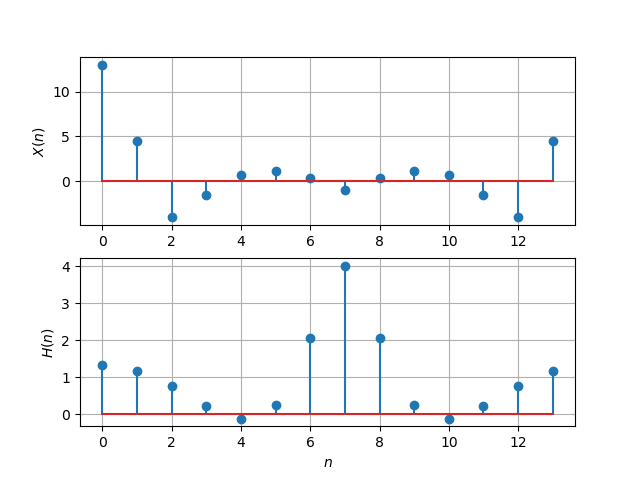
\includegraphics[width=\columnwidth]{XkHk_dft.png}
\caption{}
\label{fig:XkHk_dft}
\end{figure}
\item Express the above convolution using a Teoplitz matrix.
\\
\solution
The following code does convolution
\begin{lstlisting}
weget https://github.com/Bhanu-das/EE3900/blob/main/Assign1/codes/Q5/teoplitz.py
\end{lstlisting}
\item Show that
\begin{equation}
y(n) =  \sum_{n=-\infty}^{\infty}x(n-k)h(k)
\end{equation}
\solution from \ref{eq:convolution} ww know that
\begin{equation}
y(n) =  \sum_{k=-\infty}^{\infty}x(k)h(n-k) \label{eq:1st}
\end{equation}
now consider
\begin{equation}
    t = n-k
\end{equation}
will transform into 
\begin{equation}
y(n) =  \sum_{n-t=-\infty}^{\infty}x(n-t)h(t) \label{eq:2nd}
\end{equation}
since n is finite and $-\infty < \infty$, \ref{eq:2nd} is equivalent to 
\begin{equation}
y(n) =  \sum_{t=-\infty}^{\infty}x(n-t)h(t) \label{eq:3nd}
\end{equation}
hence proved.
\end{enumerate}

%
\section{DFT and FFT}
\begin{enumerate}[label=\thesection.\arabic*]
\item
Compute
\begin{equation}
X(k) \define \sum _{n=0}^{N-1}x(n) e^{-j2\pi kn/N}, \quad k = 0,1,\dots, N-1
\end{equation}
and $H(k)$ using $h(n)$.
\\
\solution
The following code plots
\begin{lstlisting}
weget https://github.com/Bhanu-das/EE3900/blob/main/Assign1/codes/XkHk_dft.py
\end{lstlisting}
\begin{figure}[!ht]
\centering
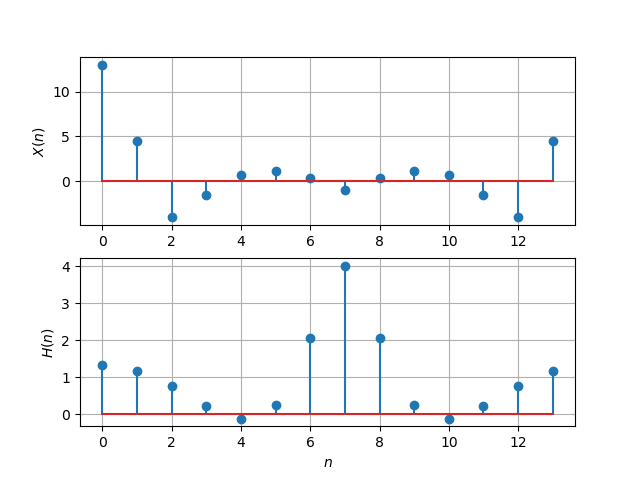
\includegraphics[width=\columnwidth]{XkHk_dft.png}
\caption{}
\label{fig:XkHk_dft}
\end{figure}
\item Compute 
\begin{equation}
Y(k) = X(k)H(k)
\end{equation}
\\
\solution
The following code plots
\begin{lstlisting}
weget https://github.com/Bhanu-das/EE3900/blob/main/Assign1/codes/yk.py
\end{lstlisting}
\begin{figure}[!ht]
\centering
\includegraphics[width=\columnwidth]{yk.png}
\caption{}
\label{fig:yk}
\end{figure}
\item Compute
\begin{equation}
 y\brak{n}={\frac {1}{N}}\sum _{k=0}^{N-1}Y\brak{k}\cdot e^{j 2\pi kn/N},\quad n = 0,1,\dots, N-1
\end{equation}
\\
\solution The following code plot. Note that this is the same as 
$y(n)$ in  Fig. 

%
\begin{lstlisting}
wget https://raw.githubusercontent.com/gadepall/EE1310/master/filter/codes/yndft.py
\end{lstlisting}
\begin{lstlisting}
weget https://github.com/Bhanu-das/EE3900-2022/blob/main/filter/figs/yndft.pdf
\end{lstlisting}

\item Repeat the previous exercise by computing $X(k), H(k)$ and $y(n)$ through FFT and  IFFT.
\\
\solution
The following code plots $X(n)$, $H(n)$ and $y(n)$ by fft.
\begin{lstlisting}
weget https://github.com/Bhanu-das/EE3900/blob/main/Assign1/codes/fft.py
\end{lstlisting}
\begin{figure}[!ht]
\centering
\includegraphics[width=\columnwidth]{fft.png}
\caption{}
\label{fig:fft}
\end{figure}


\item Wherever possible, express all the above equations as matrix equations.
\\

\solution \\
\[
\begin{array}{lc}
    x = 
  \left(\begin{array}{@{}ccc@{}}
    1 \\
    2 \\
    3 \\
    4 \\
    2 \\
    1 \\
    0 \\
    . \\
    . \\
    . \\
    0 \\
  \end{array}\right) \\[15pt]
\end{array}
\]
\[
\begin{array}{lc}
    J = 
  \left(\begin{array}{@{}ccc@{}}
    0 \\
    e^{\frac{-2\pi j(1)k}{N}} \\
    e^{\frac{-2\pi j(2)k}{N}} \\
    . \\
    . \\
    . \\
    e^{\frac{-2\pi j(N-1)k}{N}} \\
  \end{array}\right) \\[15pt]
\end{array}
\]
\begin{equation}
    X(k) = x^{T} J
\end{equation}
\[
\begin{array}{lc}
    h = 
  \left(\begin{array}{@{}ccc@{}}
    h[0] \\
    h[1] \\
    . \\
    . \\
    . \\
    h[N-1] \\
  \end{array}\right) \\[15pt]
\end{array}
\]
\begin{equation}
    H(k) = h^{T} J
\end{equation}
\[
\begin{array}{lc}
    y = 
  \left(\begin{array}{@{}ccc@{}}
    h[0] x[0] \\
    h[1] x[1] \\
    . \\
    . \\
    . \\
    h[N-1] x[N-1] \\
  \end{array}\right) \\[15pt]
\end{array}
\]
\begin{equation}
    Y(k) = y^{T} J
\end{equation} 

\item Verify the above equations by generating the DFT matrix in python.

\end{enumerate}
%
\section{FFT}
% \subsection{Definitions}
\begin{enumerate}[label=\arabic*.,ref=\thesection.\theenumi]
\numberwithin{equation}{section}
    \item The DFT of $x(n)$ is given by
    \begin{align}
        X(k) \triangleq \sum_{n=0}^{N-1} x(n) e^{-j 2 \pi k n / N}, \quad k=0,1, \ldots, N-1
    \end{align}
\item Let 
	\begin{align}
W_{N} = e^{-j2\pi/N} 
	\end{align}
		Then the $N$-point {\em DFT matrix} is defined as 
	\begin{align}
		\vec{F}_{N} = \sbrak{W_{N}^{mn}}, \quad 0 \le m,n \le N-1 
	\end{align}
	where $W_{N}^{mn}$ are the elements of $\vec{F}_{N}$.
\item Let 
	\begin{align}
\vec{I}_4 = \myvec{\vec{e}_4^{1} &\vec{e}_4^{2} &\vec{e}_4^{3} &\vec{e}_4^{4} }
	\end{align}
		be the $4\times 4$ identity matrix.  Then the 4 point {\em DFT permutation matrix} is defined as 
	\begin{align}
		\vec{P}_4 = \myvec{\vec{e}_4^{1} &\vec{e}_4^{3} &\vec{e}_4^{2} &\vec{e}_4^{4} }
	\end{align}
\item The 4 point {\em DFT diagonal matrix} is defined as 
	\begin{align}
		\vec{D}_4 = diag\myvec{W_{8}^{0} & W_{8}^{1} & W_{8}^{2} & W_{8}^{3}}
	\end{align}
\item Show that 
\begin{equation}
    W_{N}^{2}=W_{N/2}
\end{equation}
%    \item Find $\vec{P}_6$.
%    \item Find $\vec{D}_3$.
    \item Show that 
\begin{equation}
	\vec{F}_{4}=
\begin{bmatrix}
	\vec{I}_{2} & \vec{D}_{2} \\
\vec{I}_{2} & -\vec{D}_{2}
\end{bmatrix}
\begin{bmatrix}
\vec{F}_{2} & 0 \\
0 & \vec{F}_{2}
\end{bmatrix}
\vec{P}_{4}
\end{equation}
\item Show that 
\begin{equation}
\vec{F}_{N}=
\begin{bmatrix}
\vec{I}_{N/2} & \vec{D}_{N/2} \\
\vec{I}_{N/2} & -\vec{D}_{N/2}
\end{bmatrix}
\begin{bmatrix}
\vec{F}_{N/2} & 0 \\
0 & \vec{F}_{N/2}
\end{bmatrix}
\vec{P}_{N}
\end{equation}
\item Find 
    \begin{align}
	     \vec{P}_4 \vec{x}
    \end{align}
\item Show that 
    \begin{align}
	    \vec{X} = \vec{F}_N \vec{x}
	    \label{eq:dft-mat-def}
    \end{align}
		where $\vec{x}, \vec{X}$ are the vector representations of $x(n), X(k)$ respectively.
\item Derive the following Step-by-step visualisation  of
8-point FFTs into 4-point FFTs and so on
\begin{equation}
\begin{bmatrix}
X(0) \\ 
X(1) \\ 
X(2) \\ 
X(3)
\end{bmatrix}
=
\begin{bmatrix}
X_{1}(0) \\ 
X_{1}(1)\\ 
X_{1}(2)\\
X_{1}(3)\\
\end{bmatrix}
+
\begin{bmatrix}
W^{0}_{8} & 0 & 0 & 0\\
0 & W^{1}_{8} & 0 & 0\\
0 & 0 & W^{2}_{8} & 0\\
0 & 0 & 0 & W^{3}_{8}
\end{bmatrix}
\begin{bmatrix}
X_{2}(0) \\ 
X_{2}(1) \\ 
X_{2}(2) \\
X_{2}(3)
\end{bmatrix}
\end{equation}
\begin{equation}
\begin{bmatrix}
X(4) \\ 
X(5) \\ 
X(6) \\ 
X(7)
\end{bmatrix}
=
\begin{bmatrix}
X_{1}(0) \\ 
X_{1}(1)\\ 
X_{1}(2)\\
X_{1}(3)\\
\end{bmatrix}
-
\begin{bmatrix}
W^{0}_{8} & 0 & 0 & 0\\
0 & W^{1}_{8} & 0 & 0\\
0 & 0 & W^{2}_{8} & 0\\
0 & 0 & 0 & W^{3}_{8}
\end{bmatrix}
\begin{bmatrix}
X_{2}(0) \\ 
X_{2}(1) \\ 
X_{2}(2) \\
X_{2}(3)
\end{bmatrix}
\end{equation}
4-point FFTs into 2-point FFTs
\begin{equation}
\begin{bmatrix}
X_{1}(0) \\ 
X_{1}(1)\\ 
\end{bmatrix}
=
\begin{bmatrix}
X_{3}(0) \\ 
X_{3}(1)\\ 
\end{bmatrix}
+
\begin{bmatrix}
W^{0}_{4} & 0\\
0 & W^{1}_{4}
\end{bmatrix}
\begin{bmatrix}
X_{4}(0) \\ 
X_{4}(1) \\ 
\end{bmatrix}
\end{equation}
\begin{equation}
\begin{bmatrix}
X_{1}(2) \\ 
X_{1}(3)\\ 
\end{bmatrix}
=
\begin{bmatrix}
X_{3}(0) \\ 
X_{3}(1)\\ 
\end{bmatrix}
-
\begin{bmatrix}
W^{0}_{4} & 0\\
0 & W^{1}_{4}
\end{bmatrix}
\begin{bmatrix}
X_{4}(0) \\ 
X_{4}(1) \\ 
\end{bmatrix}
\end{equation}
\begin{equation}
\begin{bmatrix}
X_{2}(0) \\ 
X_{2}(1)\\ 
\end{bmatrix}
=
\begin{bmatrix}
X_{5}(0) \\ 
X_{5}(1)\\ 
\end{bmatrix}
+
\begin{bmatrix}
W^{0}_{4} & 0\\
0 & W^{1}_{4}
\end{bmatrix}
\begin{bmatrix}
X_{6}(0) \\ 
X_{6}(1) \\ 
\end{bmatrix}
\end{equation}
\begin{equation}
\begin{bmatrix}
X_{2}(2) \\ 
X_{2}(3)\\ 
\end{bmatrix}
=
\begin{bmatrix}
X_{5}(0) \\ 
X_{5}(1)\\ 
\end{bmatrix}
-
\begin{bmatrix}
W^{0}_{4} & 0\\
0 & W^{1}_{4}
\end{bmatrix}
\begin{bmatrix}
X_{6}(0) \\ 
X_{6}(1) \\ 
\end{bmatrix}
\end{equation}
\begin{equation}
P_{8}
\begin{bmatrix}
x(0) \\ 
x(1) \\ 
x(2) \\ 
x(3) \\ 
x(4) \\ 
x(5) \\
x(6) \\
x(7)
\end{bmatrix}
 = 
\begin{bmatrix}
x(0) \\ 
x(2) \\ 
x(4) \\ 
x(6) \\
x(1) \\ 
x(3) \\ 
x(5) \\
x(7)
\end{bmatrix}
\end{equation}
\begin{equation}
P_{4}
\begin{bmatrix}
x(0) \\ 
x(2) \\ 
x(4) \\ 
x(6) \\
\end{bmatrix}
 = 
\begin{bmatrix}
x(0) \\ 
x(4) \\ 
x(2) \\
x(6)
\end{bmatrix}
\end{equation}
\begin{equation}
P_{4}
\begin{bmatrix}
x(1) \\ 
x(3) \\ 
x(5) \\
x(7)
\end{bmatrix}
 = 
\begin{bmatrix}
x(1) \\ 
x(5) \\ 
x(3) \\ 
x(7) \\
\end{bmatrix}
\end{equation}
Therefore,
\begin{equation}
\begin{bmatrix}
X_{3}(0) \\ 
X_{3}(1)\\ 
\end{bmatrix}
= F_{2}
\begin{bmatrix}
x(0) \\ 
x(4) \\ 
\end{bmatrix}
\end{equation}
\begin{equation}
\begin{bmatrix}
X_{4}(0) \\ 
X_{4}(1)\\ 
\end{bmatrix}
= F_{2}
\begin{bmatrix}
x(2) \\ 
x(6) \\ 
\end{bmatrix}
\end{equation}
\begin{equation}
\begin{bmatrix}
X_{5}(0) \\ 
X_{5}(1)\\ 
\end{bmatrix}
= F_{2}
\begin{bmatrix}
x(1) \\ 
x(5) \\ 
\end{bmatrix}
\end{equation}
\begin{equation}
\begin{bmatrix}
X_{6}(0) \\ 
X_{6}(1)\\ 
\end{bmatrix}
= F_{2}
\begin{bmatrix}
x(3) \\ 
x(7) \\ 
\end{bmatrix}
\end{equation}
\item For 
    \begin{align}
	    \vec{x} = \myvec{1\\2\\3\\4\\2\\1}
        \label{eq:equation1}
    \end{align}
    compte the DFT  
		using 
	    \eqref{eq:dft-mat-def}
    \item Repeat the above exercise using the FFT
	    after zero padding $\vec{x}$.
%	    \eqref{eq:fft-mat-def}
\item Write a C program to compute the 8-point FFT. 
 \end{enumerate}
\section{Exercises}

Answer the following questions by looking at the python code in Problem \ref{prob:output}.
\begin{enumerate}[label=\thesection.\arabic*]
\item
The command
\begin{lstlisting}
	output_signal = signal.lfilter(b, a, input_signal)
	\end{lstlisting}
in Problem \ref{prob:output} is executed through the following difference equation
\begin{equation}
\label{eq:iir_filter_gen}
 \sum _{m=0}^{M}a\brak{m}y\brak{n-m}=\sum _{k=0}^{N}b\brak{k}x\brak{n-k}
\end{equation}
%
where the input signal is $x(n)$ and the output signal is $y(n)$ with initial values all 0. Replace
\textbf{signal.filtfilt} with your own routine and verify.
%
\\
\solution

\item Repeat all the exercises in the previous sections for the above $a$ and $b$.

\item What is the sampling frequency of the input signal?
\\
\solution
Sampling frequency(fs)=44.1kHZ.
\item
What is type, order and  cutoff-frequency of the above butterworth filter
\\
\solution
The given butterworth filter is low pass with order=2 and cutoff-frequency=4kHz.
%
\item
Modifying the code with different input parameters and to get the best possible output.
\\
\solution a better filtering was found on changing the order of filter to 7.
%
\end{enumerate}

\end{document}
